
\chapter{Модельный порыв}


В работе \cite{Avila2013} численно было обнаружено уникальное решение уравнений Навье-Стокса в круглой трубе. Оно воспроизводит основные особенности турбулентного порыва, но имеет более простую форму и динамику. В фазовом пространстве решение \cite{Avila2013} принадлежит сепаратрисе, разделяющей области притяжения ламинарного и турбулентного режимов течения. В круглой трубе течение Пуазейля устойчиво к малым возмущениям. Для выхода на турбулентное решение, стартуя с возмущенного течения Пуазейля, амплитуда возмущения должна быть достаточно велика. Для начального возмущения фиксированной формы можно определить такое значение амплитуды, что решение в процессе эволюции будет оставаться на сепаратрисе, разделяющей области притяжения ламинарного и турбулентного решений. Это решение неустойчиво и при численном интегрировании рано или поздно сваливается в ту или иную сторону --- либо выходит на турбулентный режим, либо возвращается к течению Пуазейля. Тем не менее, варьируя начальную амплитуду возмущения, можно проследить поведение балансирующего на сепаратрисе решения на значительном промежутке времени. Как показано в \cite{Skufca2006}, предельное решение, к которому стремится решение на сепаратрисе, сохраняет некоторые черты турбулентного решения, но при этом как правило обладает более простым поведением во времени. В \cite{Avila2013} обнаружено, что при наложении дополнительных ограничений симметрии предельное решение на сепаратрисе при $Re\sim2000$ качественно близко к турбулентному порыву, но оказывается при этом условно-периодическим по времени, а именно, периодическим в подходящей подвижной системе отсчета. Простота поведения предельного решения на сепаратрисе позволяет провести его исчерпывающее исследование и строго обосновать полученные результаты, что может быть небесполезным для понимания  механизма образования и самоподдержания турбулентных порывов. Соответствующий условно периодическому решению порыв мы будем называть {\it модельным}. Основные результаты, приведенные в этом разделе, опубликованы в работах автора диссертации \cite{MZG2015, Kazan2015}. 


\section{Получение модельного порыва} \label{edge_seq}

Следуя \cite{Avila2013}, решение поставленной в разделе \ref{math_section} задачи ищется с дополнительными ограничениями диаметральной симметричности и $\pi$-периодичности в угловом направлении:
\begin{equation}\label{sym_eq}
(v_x,v_r)(x,r,-\theta,t)=(v_x,v_r)(x,r,\theta,t),\ \ v_\theta(x,r,-\theta,t)=-v_\theta(x,r,\theta,t)
\end{equation}
\begin{equation}\label{per_eq}
(v_x,v_r,v_\theta)(x,r,\theta+\pi,t) = (v_x,v_r,v_\theta)(x,r,\theta,t)
\end{equation}
Здесь $(x, r, \theta)$ --- цилиндрические координаты, $(v_x, v_r, v_\theta)$ --- продольная, радиальная и угловая компоненты вектора скорости. Наложение ограничений \eqref{sym_eq}, \eqref{per_eq} упрощает поведение решения в пространстве, делает его более определенным. Турбулентные порывы, рассчитанные при $Re=2000$ с учетом и без учета условий \eqref{sym_eq}, \eqref{per_eq} изображены на рисунке~\ref{3D_img} (представлены области пониженной и повышенной на $0.1$ скорости относительно течения Пуазейля). В обоих случаях порыв имеет центральное ядро с пониженной скоростью и систему вытянутых вдоль стенки трубы, чередующихся в угловом направлении полос замедления и ускорения. На симметричном порыве полосы гораздо более структурированы. Их угловое положение не меняется в процессе эволюции: угловые области $\theta=k\pi/2,\ k=0-3$, где в силу \eqref{sym_eq}, \eqref{per_eq} угловая компонента скорости тождественно равна нулю, заняты полосами ускорения, промежуточные области $\theta=\pi/4+k\pi/2$ --- полосами замедления. На порыве без условий симметрии наблюдаются значительные по амплитуде случайные по пространственному расположению флуктуации, разрывающие сплошность полосчатых структур. На симметричном порыве тоже заметна флуктуирующая компонента, которая в этом случае выглядит гораздо более регулярной. Отметим, что несмотря на заметную пространственную регулярность, временн\'{о}е поведение симметричного порыва остается хаотичным.


\begin{figure}[h]
\center{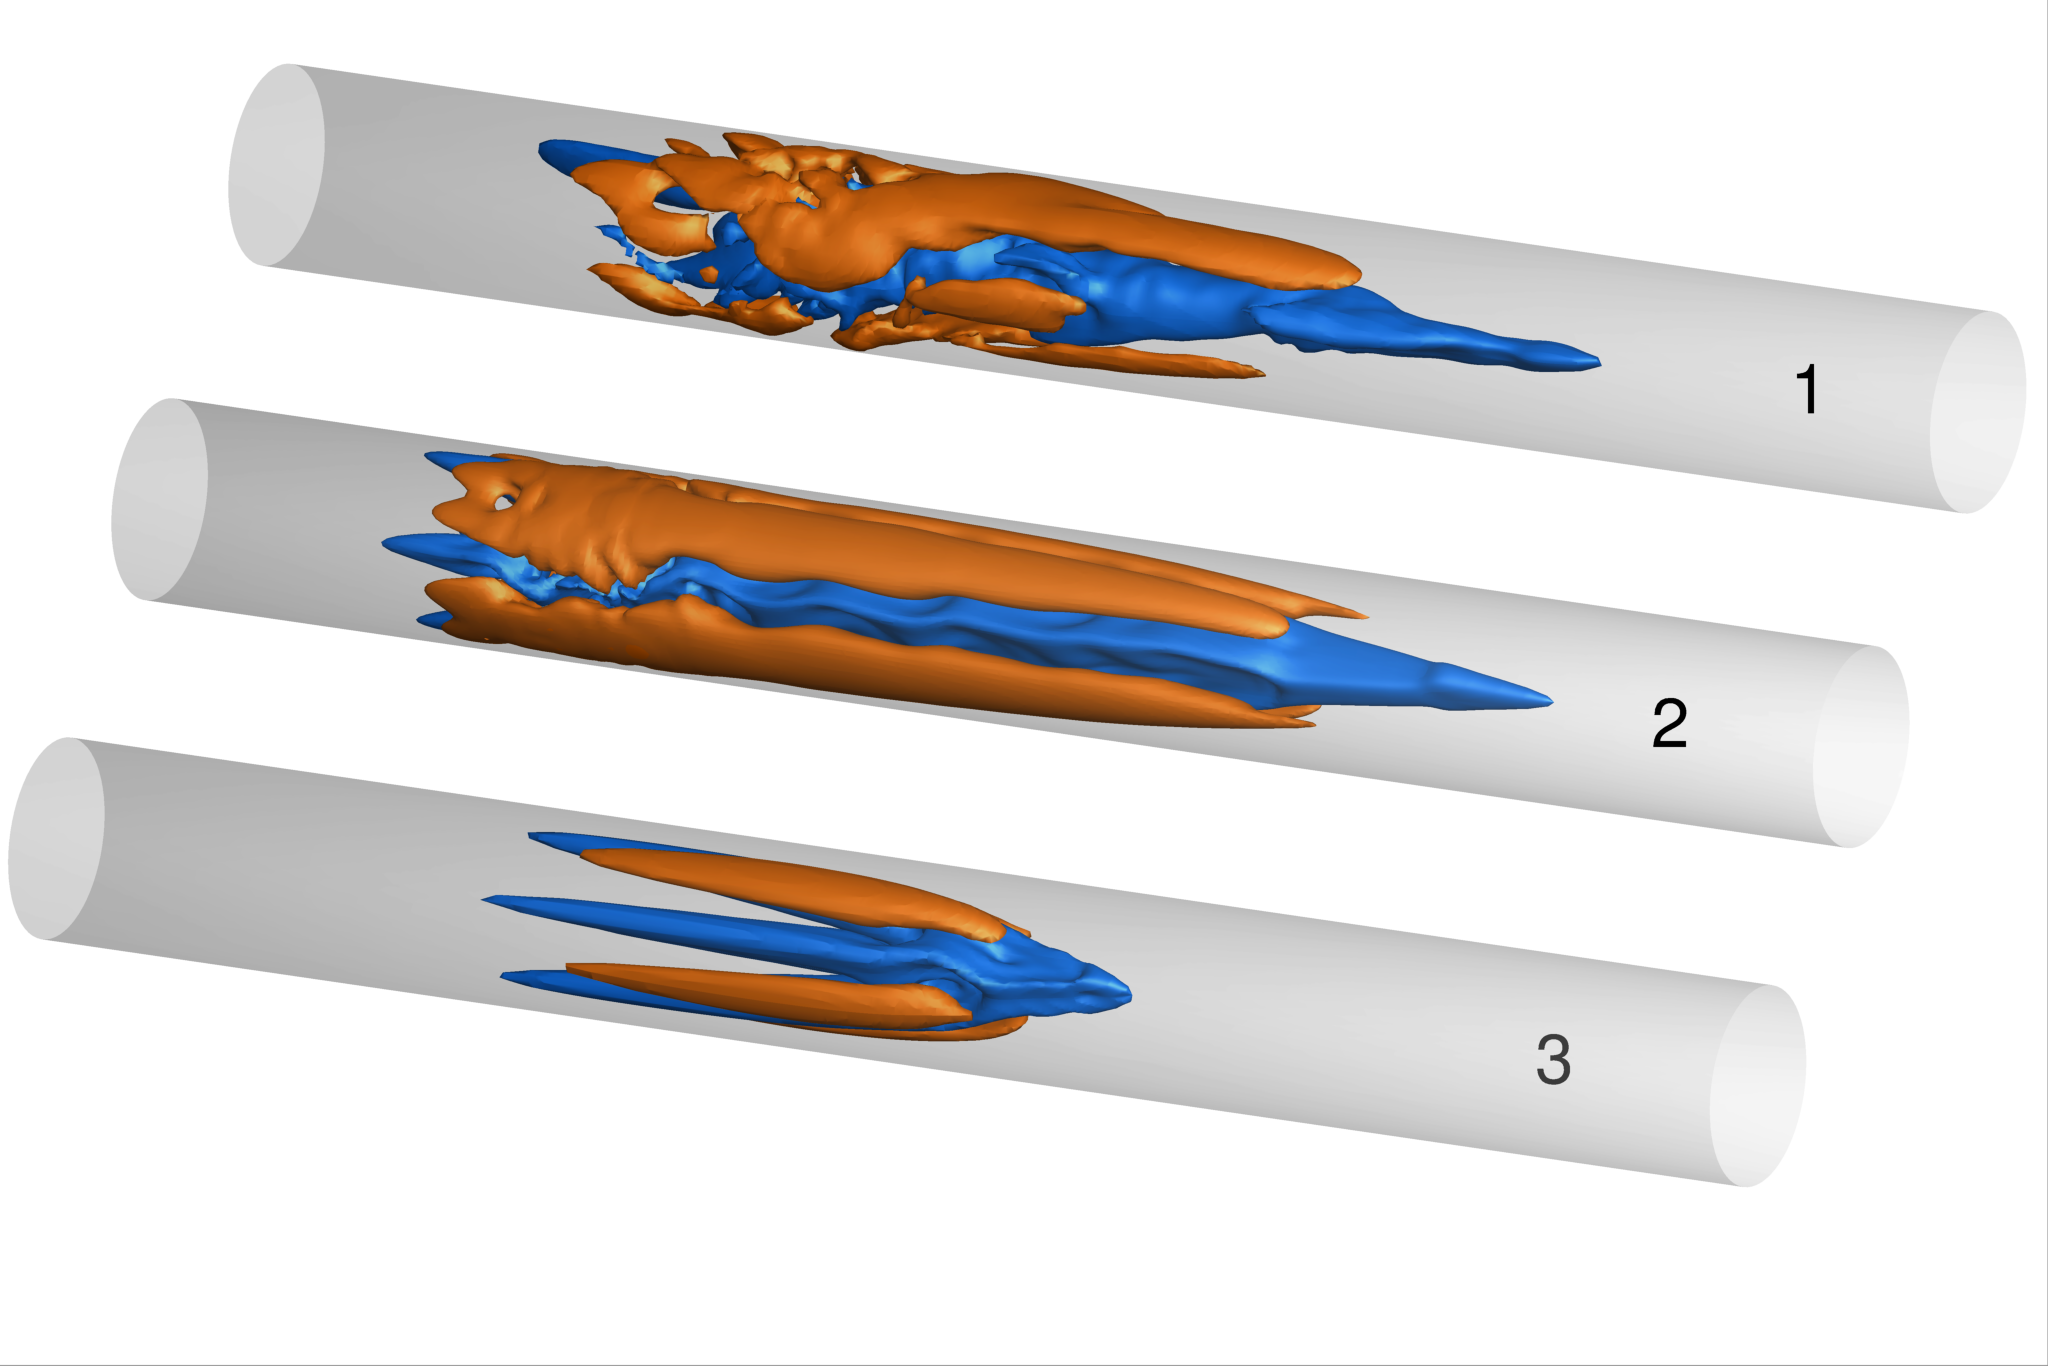
\includegraphics[width=1\linewidth]{3D_cmp.png}}
\caption{Визуализация численных расчетов турбулентных порывов: 1 --- Re = 2000; 2 --- Re = 2000 с учетом \eqref{sym_eq}, \eqref{per_eq}; 3 --- решение на сепаратрисе, Re = 2200. Синим и красным выделены поверхности скорости –0.1 и + 0.1 относительно скорости течения Пуазейля. Поток направлен слева направо.}
\label{3D_img}
\end{figure}

Предельное решение на сепаратрисе получено при $Re=2200$. Условие \eqref{per_eq} при \eqref{sym_eq} порождает условие отражения относительно сечения $\theta = \pi/2$:
\begin{equation} \label{sym2_eq}
(v_x, v_r, v_\theta)(x, r, \pi n/2 + \theta, t) = (v_x, v_r, -v_\theta)(x, r, \pi n / 2 - \theta, t).
\end{equation}
С учетом \eqref{sym_eq}, \eqref{sym2_eq} расчет проводился для четверти объема трубы $0\leqslant\theta\leqslant\pi/2$. Исходное решение найдено при $L_x = 80$ на сетке, содержащей $512 \times 32 \times  32$ ячеек в продольном, радиальном и угловом направлениях. Предварительно найденное турбулентное решение $\v_{turb}(\x,t)$ используется в итерационной процедуре отыскания предельного решения на сепаратрисе. Задача решается с начальным условием
\begin{equation} \label{edge_init_eq}
\v(\x,t=0) = \v_{Pois}(\x)+\alpha(\v_{turb}(\x,t=t_0) - \v_{Pois}(\x))
\end{equation}
Здесь $\v_{Pois}=(1-r^2,0,0)$ --- течение Пуазейля, $t_0$ --- некоторый фиксированный момент времени, $\alpha \in [0,1]$ --- скалярный параметр. Значение $\alpha=0$ соответствует нулевому возмущению, и решением при $t>0$ остается течение Пуазейля. Выбирая $\alpha=1$, мы уже в начальный момент времени попадаем на турбулентный режим и остаемся на нем при $t>0$. При промежуточных значениях $\alpha$ происходит стремление решения либо к одному, либо к другому режиму. Метод деления отрезка пополам позволяет получить значение $\alpha^*$, отделяющее те значения $\alpha$, при которых устанавливается ламинарный режим течения, от тех, при которых происходит выход на турбулентный режим. Заранее известно, что $\alpha^*$ лежит внутри отрезка $[\alpha_0', \alpha_0''] = [0,1]$. На каждой итерации длина отрезка, заключающего $\alpha^*$, сокращается вдвое. На $n$-ой итерации определяется, какой режим течения устанавливается при $\alpha_{n} = (\alpha_{n-1}' + \alpha_{n-1}'') / 2$, разделяющем отрезок $[\alpha'_{n-1}, \alpha''_{n-1}]$ на две равные части. Если устанавливается ламинарный режим течения, то $\alpha^*$ принадлежит верхней половине отрезка, $[\alpha_{n}', \alpha_{n}''] = [\alpha_{n}, \alpha_{n-1}'']$, если турбулентный --- то нижней, $[\alpha_{n}', \alpha_{n}''] = [\alpha_{n-1}', \alpha_{n}]$. На рисунке \ref{bisection_pic} представлены графики $A(t)$ --- среднеквадратичного по всему объему трубы отклонения поля скорости от течения Пуазейля для нескольких значений $\alpha_n$, демонстрирующие сходимость итерационного процесса. Уточняя значение $\alpha$, мы увеличиваем длительность балансирования решения на сепаратрисе. 


\begin{figure}[h]
\center{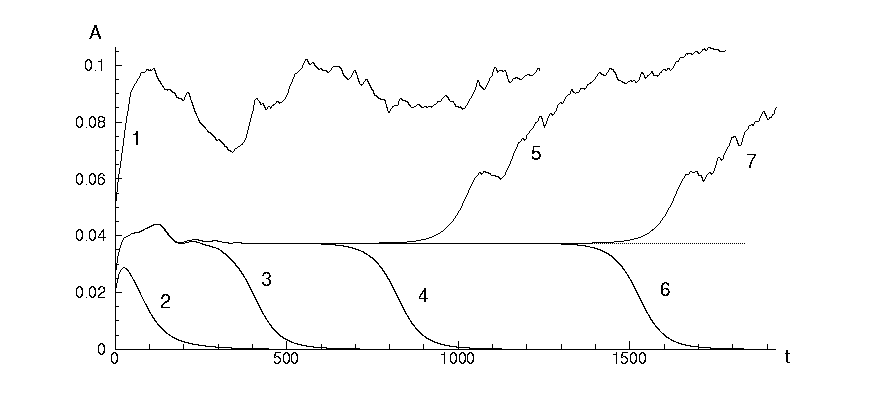
\includegraphics[width=1\linewidth]{bisection.png}}
\caption{Итерационный процесс построения решения на сепаратрисе. 1--7 --- эволюция среднеквадратичной амплитуды возмущений $A(t)$ при уточнении начального
значения.}
\label{bisection_pic}
\end{figure}

С каждой новой итерацией решение проводит на сепаратрисе в среднем на 30 временных единиц больше. При использовании 64-битных чисел с плавающей точкой для представления действительных чисел в машинном виде всего может быть сделано порядка 50 итераций, соответственно, решение можно удержать на сепаратрисе в течении приблизительно 1500 временных единиц. Из них ориентировочно первые 500 происходит перестройка решения, после чего режим течения устанавливается. В согласии с результатами \cite{Avila2013}, решение на сепаратрисе выходит на условно периодический режим. Это решение, как и турбулентный порыв, имеет форму локализованной в пространстве структуры, которая сносится вниз по потоку с постоянной скоростью. В подвижной системе отсчета поле скорости в каждой точке испытывает периодические колебания. Для скорости сноса и периода колебаний получены значения $C_f=0.69$ и $T=60$ (в \cite{Avila2013} сообщается о $C_f=0.76$ и $T=60$). Во всех выполненных расчетах режим течения, устанавливающийся на сепаратрисе, не зависит от исходного турбулентного поля скорости $\v_{turb}$. 

Так как скорость сноса модельного порыва заранее не известна, решение на сепаратрисе было найдено в системе отсчета, скорость перемещения которой была задана равной $0.5$. Для того, чтобы получить решение в сопутствующей системе отсчета, метод поиска решения на сепаратрисе применен повторно в системе отсчета, двигающейся с уже известной скоростью перемещения порыва. Когда решение на сепаратрисе найдено, изменить скорость перемещения системы отсчета уже не представляется возможным в силу высокой чувствительности решения к возмущениям, возникающим в данном случае в результате неточностей численного интегрирования. 

Сравнение предельного решения на сепаратрисе с турбулентным порывом, представленное на рисунке \ref{3D_img}, показывает качественное согласие этих решений. Во всех структурах имеются протяженные области ускоренного и замедленного движения, концентрирующиеся в пристенной области трубы. Сохраняется и основная качественная особенность порыва --- медленное понижение осевой скорости на переднем фронте и более резкое её восстановление на заднем (см. рис. \ref{ucl_cmp_img}). Мы будем называть предельное решение на сепаратрисе {\it модельным порывом}.  

\begin{figure}[h]
\center{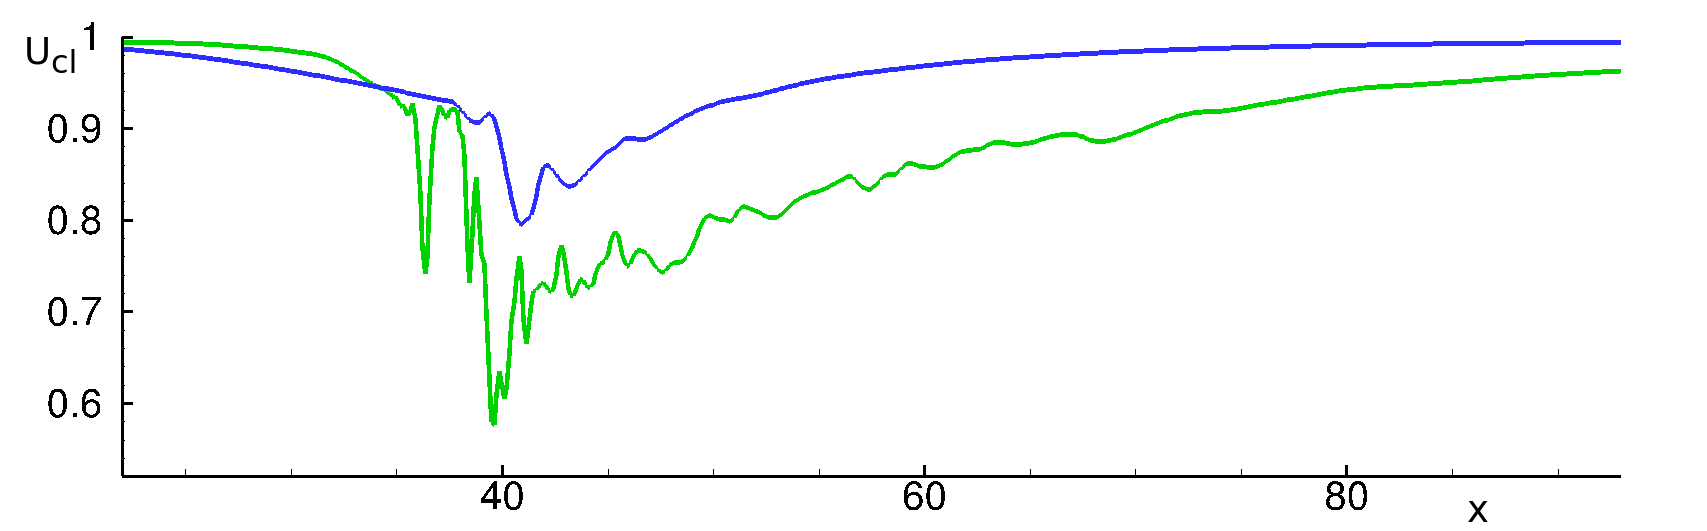
\includegraphics[width=1\linewidth]{ucl_cmp.png}}
\caption{Сравнение скорости на оси трубы в турбулентном (1) и модельном (2) порывах.}
\label{ucl_cmp_img}
\end{figure}

Результаты, полученные в расчетной области вдвое большей протяженности, при $L_x = 160$ (число узлов сетки в продольном направлении также удвоено), подтверждают локализованность предельного решения в пространстве и его независимость от условия периодичности вдоль трубы. Также, при исходном значении $L_x = 80$ решение было получено на более подробной сетке, содержащей $1024 \times 64 \times 64$ ячеек (в сравнении с исходной сеткой в каждом направлении число ячеек удвоено).  Результаты, полученные на трех сетках, близки друг к другу (см. рис. \ref{mesh_conv_pic}) и к результатам, представленным в \cite{Avila2013}. В работе \cite{Avila2013} решение получено двумя методами --- полностью спектральным \cite{Meseguer2007} и спектрально-конечно-разностным \cite{Willis2009}. В нашем случае применен конечно-разностный метод \cite{Nikitin2006}. Также, модельный порыв был воспроизведен в работе \cite{Chantry2014} спектрально-конечно-разностным методом \cite{Willis2009}; авторами также сообщается о совпадении результатов с \cite{Avila2013}. Независимость от численного метода и его параметров говорит о том, что полученное решение действительно является решением математической задачи, а не возникает в следствии неточностей численного интегрирования. 

\begin{figure}[h]
\center{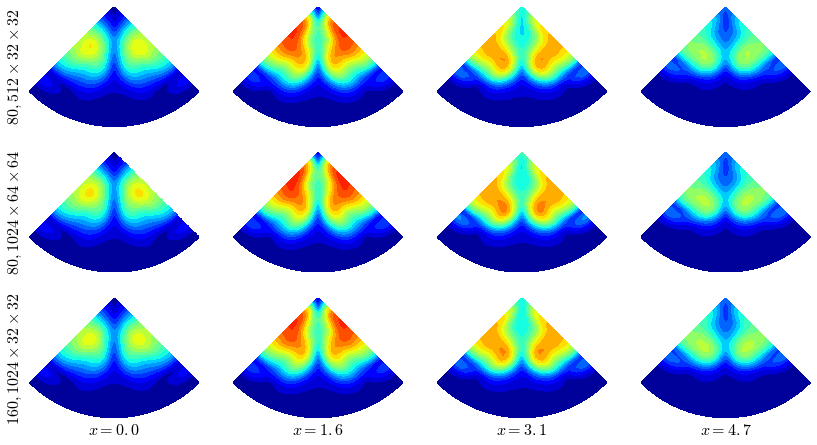
\includegraphics[width=1\linewidth]{mesh_conv.png}}
\caption{Сравнение предельного решения на сепаратрисе, полученного на нескольких расчетных сетках. Изображена интенсивность пульсаций в поперечном сечении трубы. Длина расчетной области $L_x$ и разрешение сетки, на которой получено решение, приведенное в строке, указаны слева. }
\label{mesh_conv_pic}
\end{figure}


\section{Свойства модельного порыва}

При $\Re=2200$ модельный порыв имеет длину около $40R$ и перемещается вдоль трубы с близкой к $0.69U$ скоростью. В подвижной системе отсчета он является периодическим по времени с периодом около $60 R/U$. Характерным свойством модельного порыва является наличие вытянутых вдоль потока областей с повышенным и пониженным значением продольной компоненты скорости, чередующихся в угловом направлении (см. рис. \ref{3D_img}). Полосы повышенной скорости целиком расположены около стенки трубы, полосы замедления соединяются в единое целое в приосевой области вблизи переднего фронта. Наличие вытянутых вдоль потока полос ускоренного и замедленного движения --- характерное свойство любого пристенного турбулентного течения. Однако, в отличие от реальной турбулентности, где полосы случайно блуждают во времени и в пространстве, в рассматриваемом решении полосы сохраняют свое положение и форму, лишь слегка искажаясь периодическими колебаниями. 

\begin{figure}[h]
\center{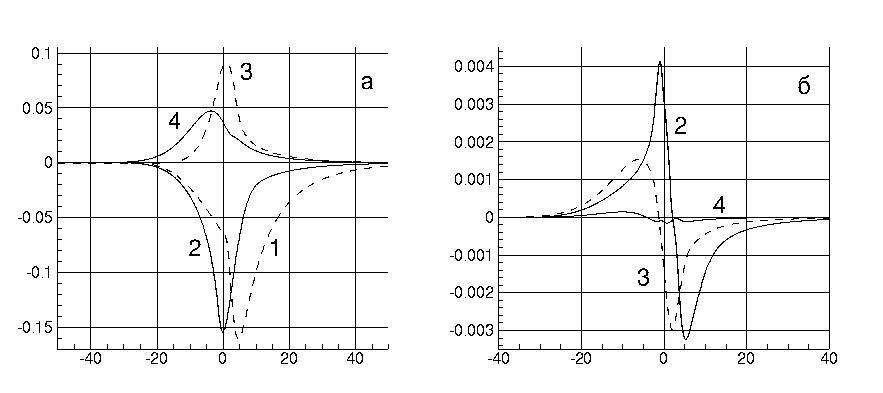
\includegraphics[width=1\linewidth]{U2D.png}}
\caption{Распределения вдоль трубы продольной (а) и радиальной (б) компоненты осесимметричной составляющей скорости $V_{2D}$ для нескольких расстояний от оси
трубы: 1–4 – r = 0, 0.4, 0.7, 0.9}
\label{U2D_pic}
\end{figure}

Для удобства перейдем в подвижную систему координат, перемещающуюся вдоль трубы со скоростью сноса локализованной структуры $c_f$. В подвижной системе решение представляется в виде суперпозиции стационарной составляющей $\V(\x) = \overline{\v}^t$ и колебательной $\v_n(t,\x) = \v - \V$. Стационарную составляющую в свою очередь представим в виде суперпозиции осесимметричной $\V_{2D}(\x) = \overline{\V}^{\theta}$ и трехмерной $\V_{3D}(\x)=\V - \V_{2D}$ составляющих. Распределения продольной компоненты осесимметричной составляющей скорости вдоль трубы $V_{x,2D}(x)$ для нескольких расстояний от оси трубы представлены на рисунке \ref{U2D_pic},а (даны отклонения от течения Пуазейля). Начало системы отсчета $x=0$ помещено в сечение, в котором среднее отклонение скорости от течения Пуазейля максимально. Голова структуры, где начинает проявляться отклонение осевой скорости, располагается на расстоянии $x \approx 45$. Хвостовая часть структуры на сепаратрисе очерчена не так четко, как в турбулентных порывах, где восстановление скорости происходит на отрезке длиной в $3-5$ радиусов трубы.  Падение скорости в приосевой области трубы компенсируется ускорением у стенки. Поведение радиальной компоненты $V_{r,2D}$, показанное на рисунке \ref{U2D_pic},б соответствует изменению осевой скорости --- в зоне замедления на оси происходит растекание жидкости к стенкам, $V_{r,2D}>0$, в передней части происходит обратный процесс и $V_{r,2D}<0$.


\begin{figure}[h]
\center{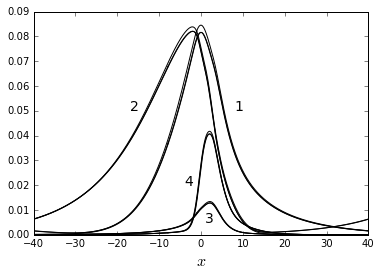
\includegraphics[width=0.5\linewidth]{amp.png}}
\caption{Распределения вдоль трубы среднеквадратичных по сечению амплитуд трех
составляющих движения: 1 – $V_{2D}$ (отклонение от течения Пуазейля); 2, 3 – продольная и поперечные компоненты скорости $V_{3D}$ ; 4 – $v_{n}$}
\label{amp_pic}
\end{figure}


На рисунке \ref{amp_pic} приведены распределения по $x$ среднеквадратичных по сечению трубы амплитуд трех составляющих движения: стационарной осесимметричной (отклонение от течения Пуазейля) $A_{2D}$, стационарной трехмерной $A_{3D}$ и колебательной $A_n$. Распределение $A_{2D}(x)$ соответствует рисунку \ref{U2D_pic}. Отклонение от течения Пуазейля заметно на значительном отрезке от $x=-30$ до $x=40$. Максимум $A_{2D}$ составляет 8.4\%. Величина $A_{3D}$ характеризует интенсивность полосчатых структур. Как видно на фиг.~\ref{3D_img} полосчатые структуры появляются на некотором расстоянии вверх по потоку от головы порыва и сохраняются на значительном расстоянии позади него. В согласии с этим $A_{3D}(x)$ имеет выраженную асимметрию относительно точки $x=-2$, где эта величина достигает максимума. Интенсивность полос быстро падает вниз по потоку и сохраняется на значительном расстоянии в верхней части потока. В отличие от стационарных полосчатых структур, колебательная составляющая движения сосредоточена на сравнительно непротяженном отрезке трубы от $x=-5$ до $x=15$ с максимальной амплитудой в 4\% при $x=2.5$.


\begin{figure}[h]
\center{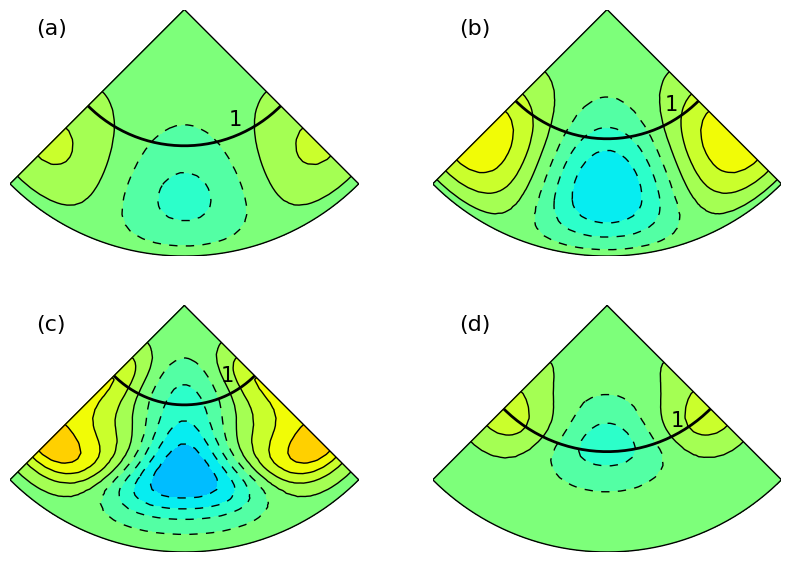
\includegraphics[width=0.8\linewidth]{V3D_cs.png}}
\caption{Распределения скорости полосчатых структур в нескольких сечениях трубы:
а–г --- x = –20, –10, 0, 5. Темный фон --- отрицательная скорость, светлый фон --- положительная скорость; 1 – линии нулевой скорости осесимметричной составляющей движения. В сечении (в) изображено векторное поле поперечного движения.}
\label{V3D_cs_pic}
\end{figure}


В трехмерную стационарную составляющую движения $V_{x,3D}$ попадают полосы повышенной и пониженной скорости. Поле $V_{x,3D}$ в нескольких сечениях трубы изображено на рисунке~\ref{V3D_cs_pic}. В каждом сечении трубы полосы пониженной скорости ($V_{x,3D} < 0$) проходят через центр расчетной области, при $\theta = \pi/4$. Полосы повышенной скорости ($V_{x,3D} > 0$) попадают на границы расчетной области в угловом направлении, находящиеся при $\theta = 0, \pi/2$. Среднее поле скорости оказывается симметрично относительно плоскости, проходящей через центр расчетной области при $\theta = \pi/4$, так как поле скорости решения на сепаратрисе $\v$ имеет дополнительную симметрию отражения относительно указанной плоскости со сдвигом на половину периода по времени:
\begin{equation}
(v_x, v_r, v_\theta)(x, r, \pi/4 + \theta, t) = (v_x, v_r, -v_\theta)(x, r, \pi/4 - \theta, t + T/2). 
\end{equation} 


\begin{figure}[h]
\center{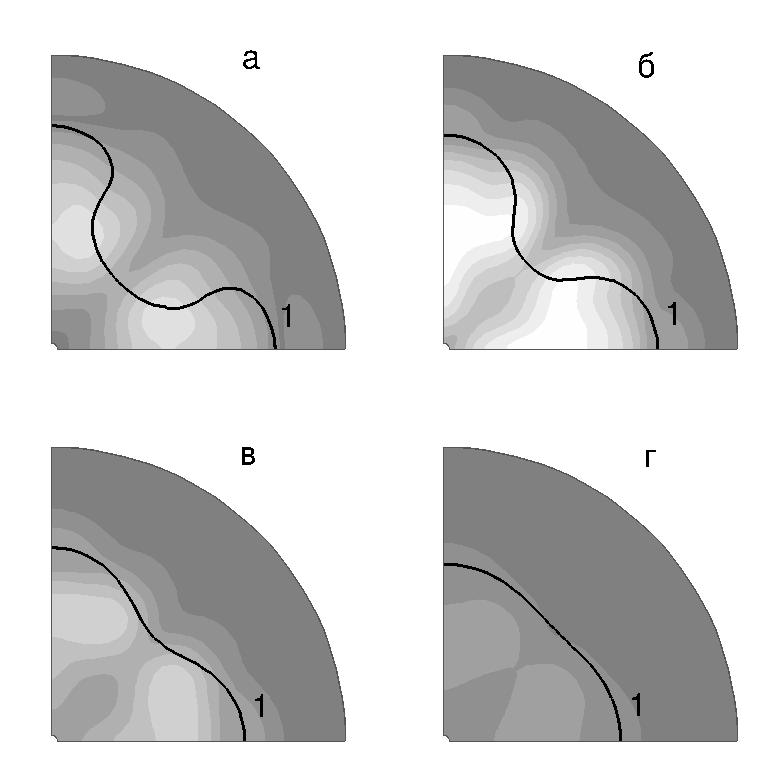
\includegraphics[width=0.8\linewidth]{puls_cs.png}}
\caption{Распределения среднеквадратичной амплитуды колебаний в нескольких сечениях трубы: а--г --- x = 0, 2.5, 5, 7.5. Максимальные значения выделены светлым
тоном. 1 – линия нулевой скорости относительного движения.}
\label{puls_cs_pic}
\end{figure}


Распределения среднеквадратичной амплитуды колебаний в нескольких сечениях трубы приведены на рисунке \ref{puls_cs_pic}. Основные колебания оказываются сосредоточены между полосами повышенной и пониженной скорости, а также между полосой ускорения и осью трубы. Пульсационная составляющая движения $\v_n$ представляет собой бегущую вниз по порыву волну, представленную в первую очередь периодическим смещением полосы пониженной скорости в угловом направлении. На рисунке~\ref{puls_ls_pic} изображено поле скорости $v_{x,n}$ в сечении $\theta = 0$ в четыре момент времени, равномерно распределенные по одному периоду изменения решения во времени. Хотя длина бегущей волны, соответствующей пульсационной составляющей движения, несколько меняется по мере продвижения вниз по трубе, её можно оценить в $5R$, а скорость её перемещения вниз по потоку в $0.77U$, что на $0.08U$ выше скорости перемещения порыва вниз по трубе.  


\begin{figure}[h]
\center{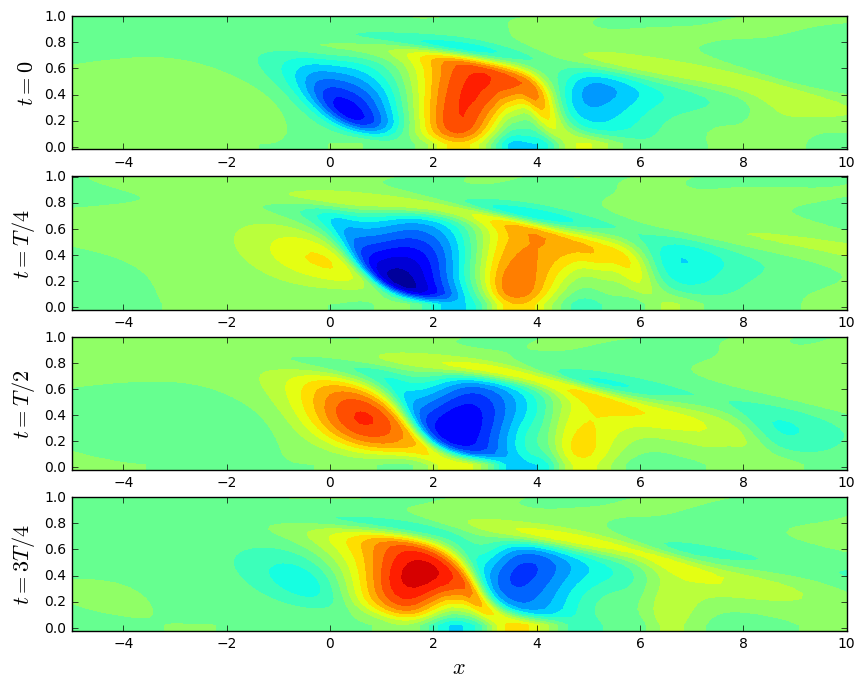
\includegraphics[width=0.8\linewidth]{v1_ls.png}}
\caption{Значение $v_{x,n}$ в сечении $\theta=0$ в моменты времени $0, T/4, T/2, 3T/4$. Синий --- отрицательное значение скорости, зеленый --- нулевое, красный --- положительное. Пульсационная составляющая движения перставляет собой бегущую вниз по потоку волну. }
\label{puls_ls_pic}
\end{figure}


\section{Механизм образования полос повышенной и пониженной скорости} 

Все описанные составляющие движения находятся в динамическом взаимодействии друг с другом. Как видно на рисунке \ref{amp_pic} наиболее локализованной вдоль трубы оказывается колебательная составляющая. Распределения среднеквадратичной амплитуды колебаний в нескольких сечениях трубы приведены на рисунке \ref{puls_cs_pic}.  Доминирующая мода колебательной составляющей пропорциональна $\exp(2\pi it/T)$ во времени и $\exp(2i\theta)$ в угловом направлении. Нелинейное взаимодействие колебательных мод порождает колебания на высших частотах, а также дает вклад в стационарную составляющую движения. В стационарной составляющей кроме осесимметричной части доминирует мода, пропорциональная $\exp(4i\theta)$, то есть с периодом $\pi/2$ в угловом направлении. Именно такой периодичности по углу соответствуют четыре пары полосчатых структур, наблюдающихся при решении задачи с условиями \eqref{sym_eq}, \eqref{per_eq}.

Отметим, что непосредственный вклад колебаний в образование полос не велик. Основной механизм роста полос это так называемый лифтап (<<lift-up>>) эффект, связанный с появлением движения в перпендикулярной к основному потоку плоскости. Частицы жидкости, перемещающиеся от стенки в сторону оси трубы, приносят дефект скорости и образуют полосу замедления, а частицы двигающиеся в противоположном направлении --- от оси к стенке, образуют полосу ускорения. Основная роль колебательной составляющей в этом механизме состоит именно в порождении стационарного движения в поперечной плоскости, распределение среднеквадратичной амплитуды которого $A_\bot(x)$ также представлено на рисунке \ref{amp_pic}. Как видно, область сосредоточения поперечного движения практически совпадает с областью существования колебаний. Некоторое уклонение $A_\bot(x)$ в заднюю сторону объясняется конвективным переносом этого движения (поперечное движение в основном возникает в периферийной части сечения трубы, где скорость потока в выбранной системе отсчета отрицательна).

Стационарное поперечное движение направлено от оси трубы к стенке в областях $\theta=k\pi/2$ и наоборот, от стенки к оси в промежуточных областях $\theta=\pi/4+k\pi/2$. Соответственно, в первых возникают полосы ускорения, во вторых --- замедления. Распределения скорости полосчатых структур в нескольких сечениях трубы приведены на рисунке \ref{V3D_cs_pic}. В сечении $x=0$, где максимальна (среди сечений, представленных на рисунке~7) интенсивность поперечного движения, изображено также векторное поле поперечного движения, демонстрирующее лифт-ап механизм образования полосчатых структур. На всех сечениях рисунка~\ref{V3D_cs_pic} сплошной линией изображена линия нулевой скорости осесимметричной составляющей движения в подвижной системе отсчета. В приосевой области, ограниченной этой линией, скорость положительна, а в периферийной --- отрицательна. Как видно из рисунков, полосчатые структуры во всех сечениях кроме самого переднего из представленных ($x=5$) располагаются в области отрицательной относительной скорости. Осесимметричное движение с отрицательной скоростью переносит полосчатые структуры в заднюю часть порыва, где они формируют картину, похожую на вытянутые щупальца медузы (см. рис.~\ref{3D_img}). При $x>5$ полосчатые структуры концентрируются в приосевой части трубы и конвектируются вперед положительной скоростью относительного движения, благодаря чему в передней части порыва $A_{3D}$ сохраняет заметную величину, несмотря на отсутствие поперечного движения.


\section{Механизм образования пульсационной составляющей движения}

\begin{figure}[h]
\center{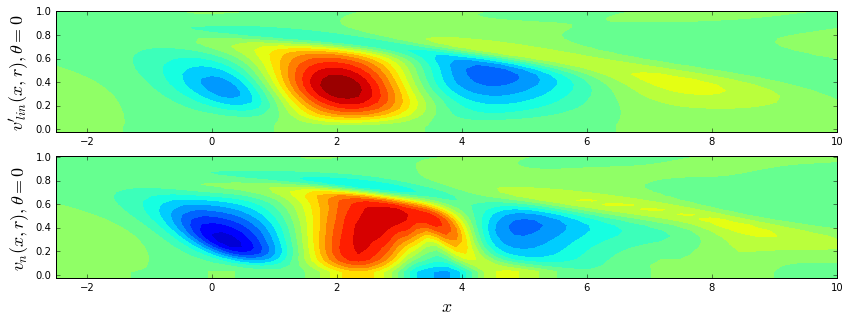
\includegraphics[width=1\linewidth]{lin_ls_cmp.png}}
\caption{Сравнение мгновенного поля продольной скорости пульсаций, возникающих в рамках линеаризованных уравнений \eqref{lin_eq}, $\v'_{lin}$ (вверху) и пульсационной составляющей движения $\v_n$ (внизу) в сечении $\theta = 0$.}
\label{lin_ls_cmp_pic}
\end{figure}

Полосчатые структуры достигают максимальной амплитуды в области $x\in[-5,0]$, где создаются условия для возникновения колебаний. Наиболее вероятный механизм генерации колебаний --- механизм потери устойчивости стационарной составляющей течения. Для проверки этой гипотезы стационарное течение $\V$ было исследовано на устойчивость к малым возмущениям $\v'$. Предположение малости $\v'$ позволяет линеаризовать уравнения. Линеаризованное уравнение Навье-Стокса имеет вид: 
\begin{equation} \label{lin_eq}
\frac{\partial \v'}{\partial t} = c_f \frac{\partial \v'}{\partial x} - \i D' - (\V, \nabla) \v' - (\v', \nabla) \V - \nabla p' + \frac{1}{\Re} \nabla^2 \v',
\end{equation}
Штрихом обозначены пульсационные составляющие соответствующих величин. Расход $\v'$ равен нулю. Другие уравнения в постановке задачи линейные и не меняют свой вид. 

Линеаризованные относительно возмущений уравнения с некоторыми случайными начальными условиями интегрировались по времени до выхода решения на режим экспоненциального изменения. Обнаружено, что действительно поле скорости $\V$ неустойчиво к малым возмущениям. Растущее возмущение $\sim\exp(\lambda+i\omega)t$ имеет коэффициент роста $\lambda=0.012$ и частоту $\omega=0.116$, близкую к частоте колебаний $2\pi/60=0.105$ в решении на сепаратрисе. Что еще более существенно, распределение амплитуды колебаний в растущем решении задачи линейной устойчивости оказывается близким к соответствующим распределениям колебательной составляющей решения на сепаратрисе (см. рис. \ref{lin_ls_cmp_pic}, \ref{lin_amp_cmp_pic}). Таким образом, нет сомнений, что механизмом появления колебаний является линейная неустойчивость стационарной составляющей движения. 

\begin{figure}[h]
\center{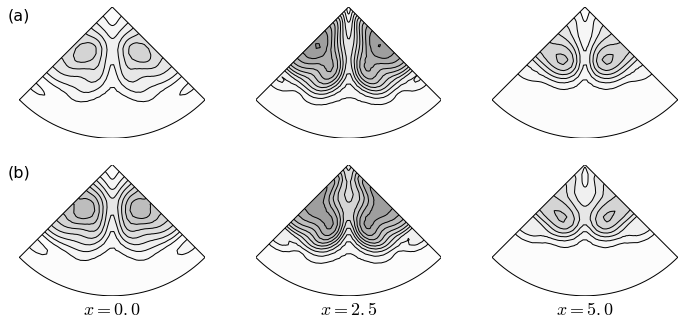
\includegraphics[width=1\linewidth]{lin_amp_cmp.png}}
\caption{Сравнение амплитуды пульсаций, возникающих в рамках линеаризованных уравнений \eqref{lin_eq}, $\v'_{lin}$ (вверху) и пульсационной составляющей движения $\v_n$ (внизу) в нескольких сечения трубы.}
\label{lin_amp_cmp_pic}
\end{figure}

Отметим, что неустойчивость полосчатых структур является неотъемлемой составляющей всех сценариев самоподдержания турбулентности в пристенных течениях. При этом чаще всего предполагается, что неустойчивость возникает в пристенных областях полос замедленного движения, где в локальном профиле скорости $V(r)$ на фоне наибольшего градиента появляется точка перегиба --- источник неустойчивости в механизме типа Кельвина--Гельмгольца. В частности, именно такой механизм предлагается в качестве механизма возникновения колебаний в турбулентном порыве в \cite{Shimizu2009}. В рассматриваемом нами решении на сепаратрисе это определенно не так. Как видно на фиг.~6 в сечении $x=0$, соответствующем максимальной скорости роста колебаний, амплитуда колебаний минимальна как раз в области полосы замедления ($\theta=\pi/4$). Наибольшие колебания развиваются наоборот вблизи полос ускорения, а если быть более точным, в промежуточных областях между полосами. В этих областях стационарная составляющая скорости течения претерпевает наибольшее изменение и имеет точки перегиба, но не как функция радиальной переменной, а как функция угла. Во всех сечениях фиг.~\ref{puls_cs_pic} сплошными линиями изображены линии нулевой относительной скорости стационарной составляющей течения. Видно, что в сечении $x=0$, где происходит основной рост колебаний, в областях максимальной амплитуды колебаний наблюдается наиболее быстрое изменение скорости как функции угловой переменной.

Отметим также, что точки максимального роста колебаний находятся на линии $r\approx0.4$, что соответствует нулевой относительной скорости. По этой причине область порождения колебаний остается неподвижной относительно порыва. Интересно, что в этой же области ($x=0,\ r\approx0.4$) происходит смена знака радиальной компоненты осесимметричной составляющей скорости (см. фиг.~4,б). При $x<0$ радиальная скорость положительна, поэтому колебания, возникшие в задней части порыва, относятся в сторону стенки трубы, где относительная скорость отрицательна, и уносятся в хвостовую часть порыва. Наоборот, при $x>0$ радиальная скорость направлена к оси трубы, туда же, в область положительной скорости, сносятся и колебания, обнаруживающиеся в передней части порыва.


\section{Влияние продольной неоднородности среднего поля скорости на форму пульсаций}

Интересно отметить, что область наибольшей интенсивности пульсаций совпадает с областью резкого изменения скорости на оси трубы (см. рис. \ref{ucl_cmp_img}, \ref{amp_pic}). Аналогичную особенность выделяют также в турбулентном порыве \cite{Hof2010}. Для того, чтобы установить влияние продольной неоднородности стационарного течения на образование пульсаций, было исследовано на устойчивость однородное вдоль трубы поле скорости $\U$, воспроизводящее полосчатые структуры. В этом случае коэффициенты в уравнении \eqref{lin_eq} не зависят от $x$, и собственные решения могут быть представлены в виде $\v' = \hat \v(r,\theta,t) \exp(i \alpha x)$, что позволяет исключить переменную $x$ из постановки задачи. Уравнение \eqref{lin_eq} в этом случае принимает вид:
\begin{equation*}
\frac{\partial \hat v_x}{\partial t} =  i \alpha (c_f - U_x) \hat v_x - \hat d - i \alpha \hat p - (\U_{\perp},\nabla_{\perp}) \hat v_x - 
(\hat \v_{\perp}, \nabla) U_x  + \frac{1}{\Re}( \nabla_{\perp}^2 - \alpha^2 ) \hat v_x,
\end{equation*}
\begin{equation*}
\frac{\partial \hat \v_{\perp}}{\partial t} = i \alpha (c_f - U_x) \hat \v_{\perp}  - \nabla_{\perp} \hat p - (\U_{\perp},\nabla_{\perp}) 
\hat \v_{\perp} - (\hat \v_{\perp}, \nabla) \U_{\perp} + \frac{1}{\Re}( \nabla_{\perp}^2 - \alpha^2 ) \hat \v_{\perp}, 
\end{equation*}
где $\perp$ обозначает проекцию соответствующей величины в плоскости поперечного сечения трубы, ортогональную $x$. Все величины, отмеченные крышечкой, комплексные и не зависят от $x$. Также меняет свой вид уравнение неразрывности:
\begin{equation*}
\nabla_{\perp} \cdot \hat \v_{\perp} = - i \alpha \hat v_x. 
\end{equation*}


\begin{figure}[h]
\center{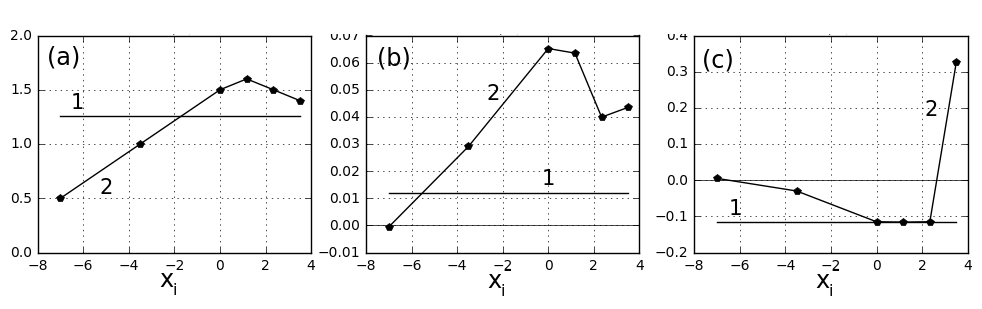
\includegraphics[width=1\linewidth]{cs_lin.png}}
\caption{Значение волнового числа $\alpha$, инкремента нарастания $\lambda$ и фазовой скорости $c_f$ для наиболее быстрорастущего собственного возмущения, возникающего на однородном вдоль трубы поле скорости, повторяющем среднее поле скорости в сечении $x$ (синий) и пульсационной составляющей движения $\v_n$ (красный).}
\label{cs_lin_pic}
\end{figure}



Однородное вдоль трубы поле скорости $\V$ создавалось 
Было выбрано несколько сечений трубы, среднее поле скорости в которых было использовано для создания однородного вдоль трубы поля $\V$. 

 
\begin{figure}[h]
\center{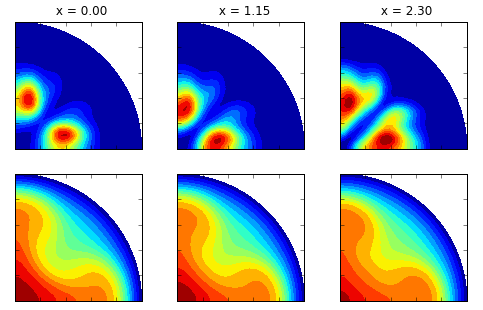
\includegraphics[width=0.8\linewidth]{cs_lin_map.png}}
\caption{Сверху приведена амплитуда пульсаций наиболее быстрорастущего возмущения, возникающего на однородном вдоль трубы поле скорости, изображенном ниже. Однородное поле скорости повторяет среднее поле скорости в сечении $x$, указанном над иллюстрациями.}
\label{cs_lin_map_pic}
\end{figure}

\section{Энергетический баланс между компонентами движения модельного порыва}



\section{Обсуждение результатов}

Общепринято, что непременным атрибутом цикла самоподдержания турбулентности в пристенных течениях являются полосчатые структуры --- долгоживущие конечноамплитудные образования, возникающие в пристенных областях. Рассмотренные в данной работе пространственно-локализованные турбулентные порывы также обладают полосчатыми структурами, что свидетельствует о вероятной близости механизма их самоподдержания с механизмом самоподдержания однородной (нелокализованной) пристенной турбулентности. Изучено численное решение уравнений Навье--Стокса, аппроксимирующее течение в турбулентном порыве. Это предельное решение на сепаратрисе, разделяющей области притяжения ламинарного и турбулентного решений. Простота временного поведения этого решения позволяет провести исчерпывающее исследование механизма его самоподдержания. На рассмотренном примере подтверждена определяющая роль полосчатых структур. Наглядно показан процесс образования вытянутых полос, включающий действие лифтап  эффекта на ограниченном отрезке длины с последующим конвективным растяжением вдоль стенки трубы. Наиболее важный результат проведенного исследования состоит в том, что обнаруженная неустойчивость полосчатого движения противоречит общепринятой точке зрения, согласно которой доминирующей является неустойчивость Кельвина--Гельмгольца, возникающая в пристенных областях полос замедленного движения. В рассмотренном примере уровень колебаний в области полос замедления минимален. Генерация колебаний происходит в промежуточной области между полосами на фоне резкого изменения скорости вдоль угловой координаты. Для выяснения деталей механизма обнаруженной неустойчивости планируется более подробное исследование. Вопрос о степени приложимости сделанных выводов к течению в турбулентном порыве и другим турбулентным течениям остается за рамками данного исследования и находится в настоящее время в стадии изучения.


